\documentclass[11pt]{article}

\usepackage[margin=1in]{geometry}
\usepackage{amsmath}
\usepackage{booktabs}
\usepackage{float}
\usepackage{graphicx}
\usepackage[hidelinks]{hyperref}
\usepackage{xcolor}

\graphicspath{{figures/}}
\setlength{\parindent}{0pt}
\setlength{\parskip}{0.65em}

\title{Class Activity 1.9: Cliff Walking with SARSA}
\author{Aispur Santiago \quad Amaya Bryan\\[0.5em]
\normalsize Course: Intelligent Agents\\
\normalsize Instructor: PhD Armas Rolando}
\date{\today}

\begin{document}
\maketitle

\section{Method}

We implemented the $4\times12$ deterministic Cliff Walking environment and
tabular SARSA from scratch.  The action-value table has shape
$4\times12\times4$ and is initialized to zero.  For a nonterminal transition,
the update is
\[
Q(S_t,A_t) \leftarrow Q(S_t,A_t) + \alpha
\left[R_{t+1}+\gamma Q(S_{t+1},A_{t+1})-Q(S_t,A_t)\right].
\]
The behavior policy is $\epsilon$-greedy.  Exploration selects uniformly among
all four actions, while exploitation selects uniformly among the maximizing
actions so that initial ties are unbiased.  Unless otherwise stated,
$\alpha=0.5$, $\gamma=1$, $\epsilon=0.1$, and training lasts 500 episodes with
a 1,000-step cap.  Curves are averages over 50 independent runs using seeds
0--49, followed by a 10-episode moving average.  NumPy implements the
environment and learner; Matplotlib is used only for figures.

\section{Results}

\begin{figure}[H]
  \centering
  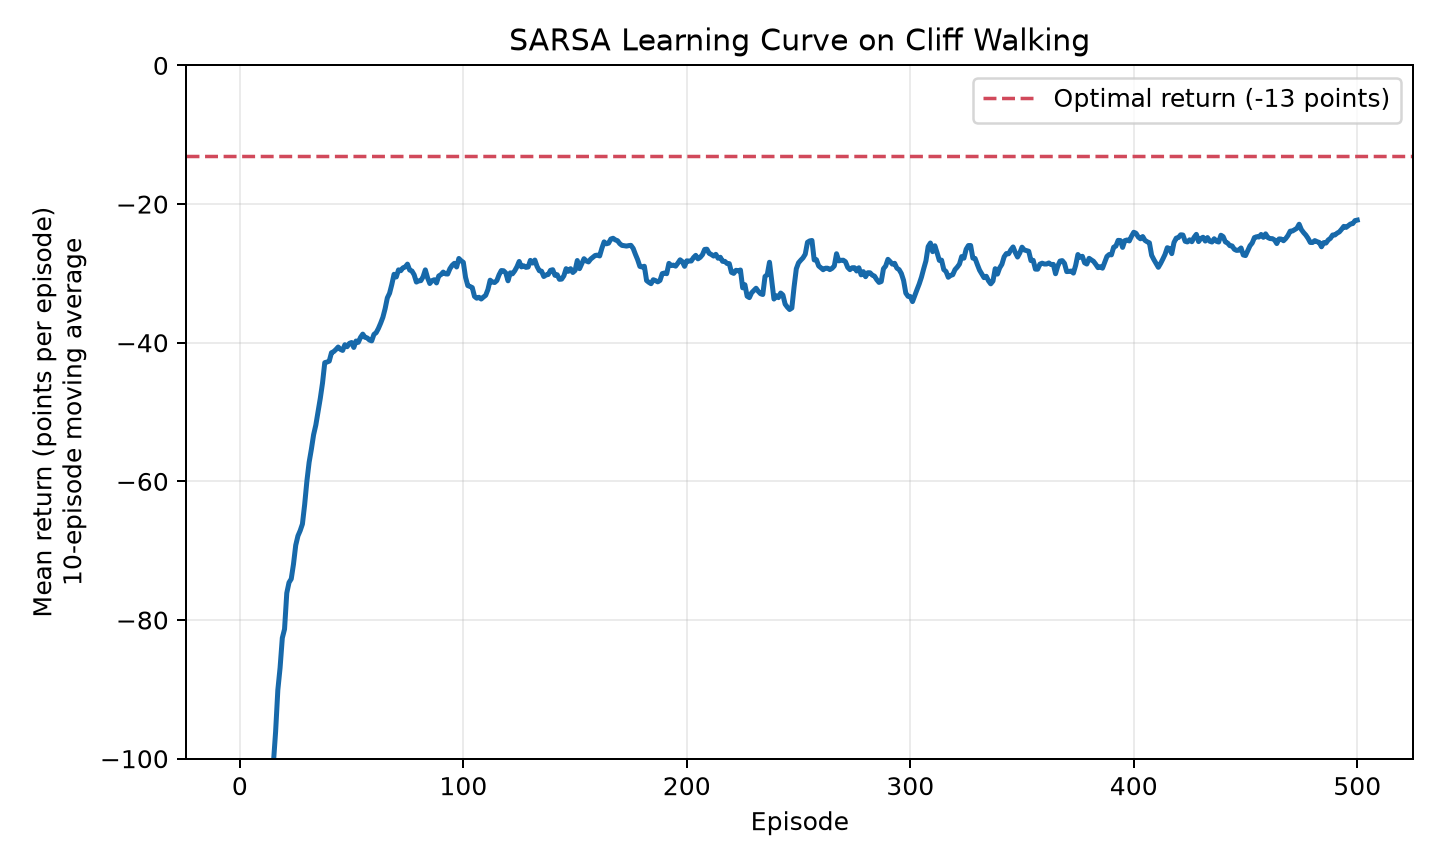
\includegraphics[width=0.92\linewidth]{learning_curve.png}
  \caption{Mean return per episode over 50 runs for $\epsilon=0.1$, smoothed
  with a trailing 10-episode moving average (shorter windows are used for the
  first nine points).  The displayed range is limited to $[-100,0]$; early
  episodes fall below the lower limit.}
  \label{fig:learning}
\end{figure}

The learning curve improves sharply during the first part of training and
then fluctuates around a stable level.  The remaining gap from $-13$ is
expected because the plotted values are returns generated by an exploratory
policy, not evaluations of a purely greedy policy.

\begin{figure}[H]
  \centering
  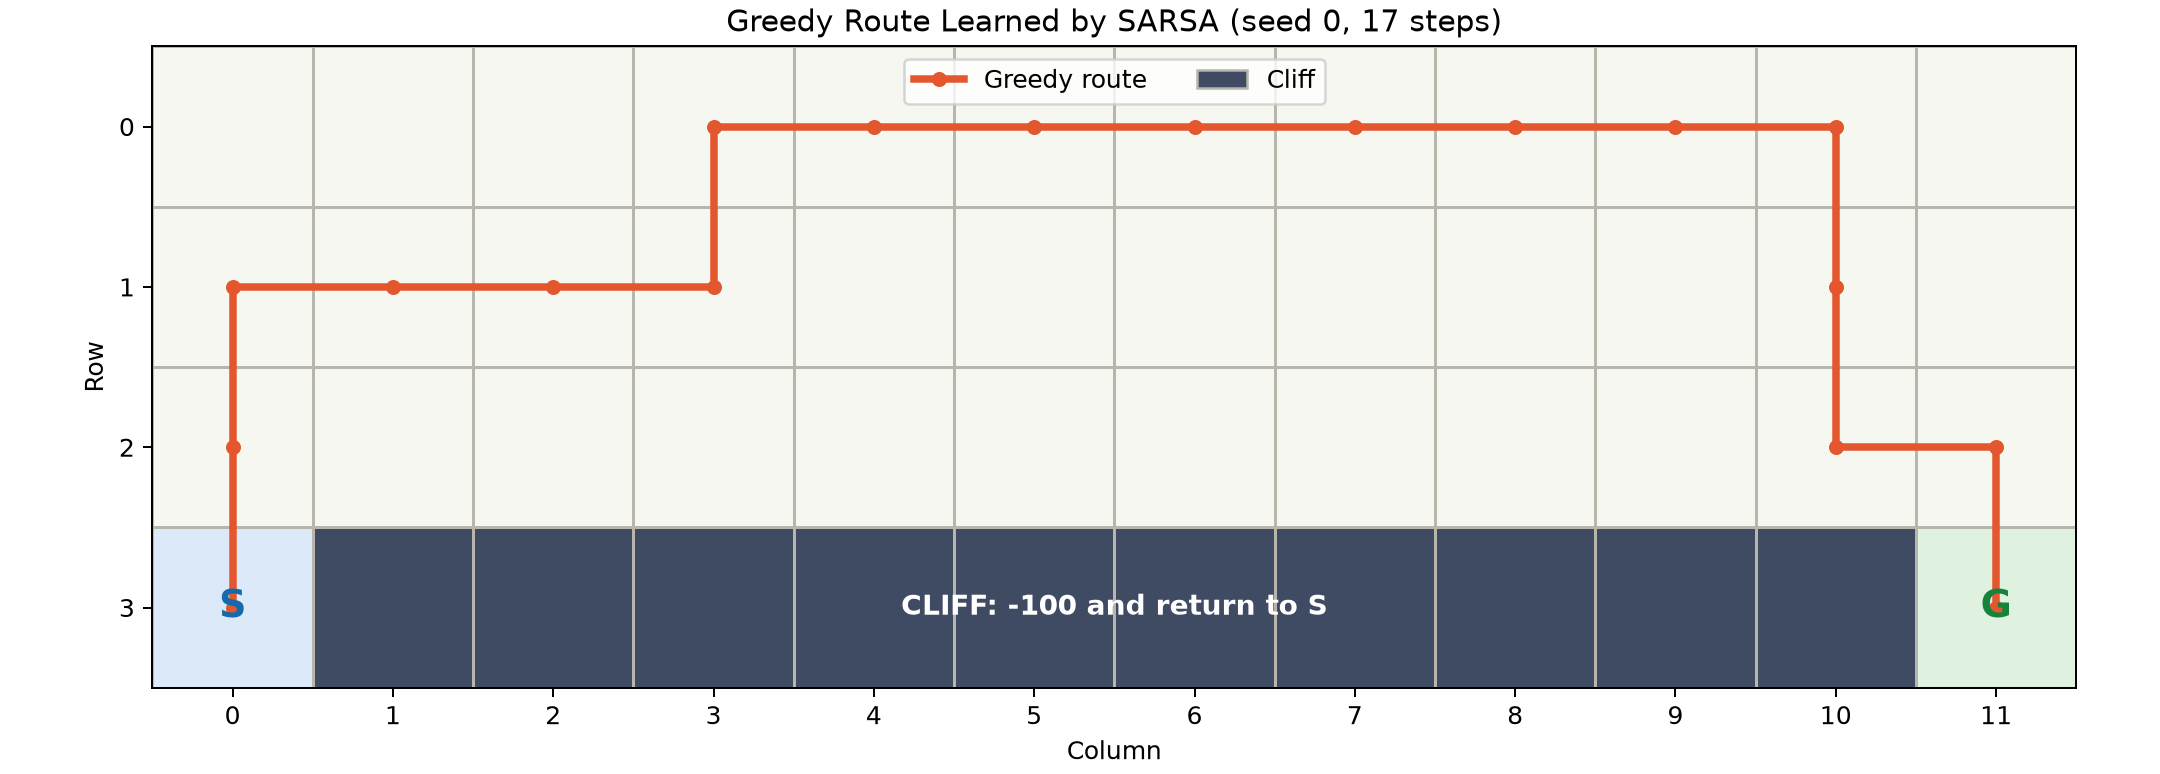
\includegraphics[width=\linewidth]{greedy_path.png}
  \caption{Greedy route extracted from the seed-0 Q-table after 500 episodes.
  The 17-step policy moves away from the cliff, crosses mainly along the top
  of the grid, and descends near the goal.}
  \label{fig:path}
\end{figure}

\begin{figure}[H]
  \centering
  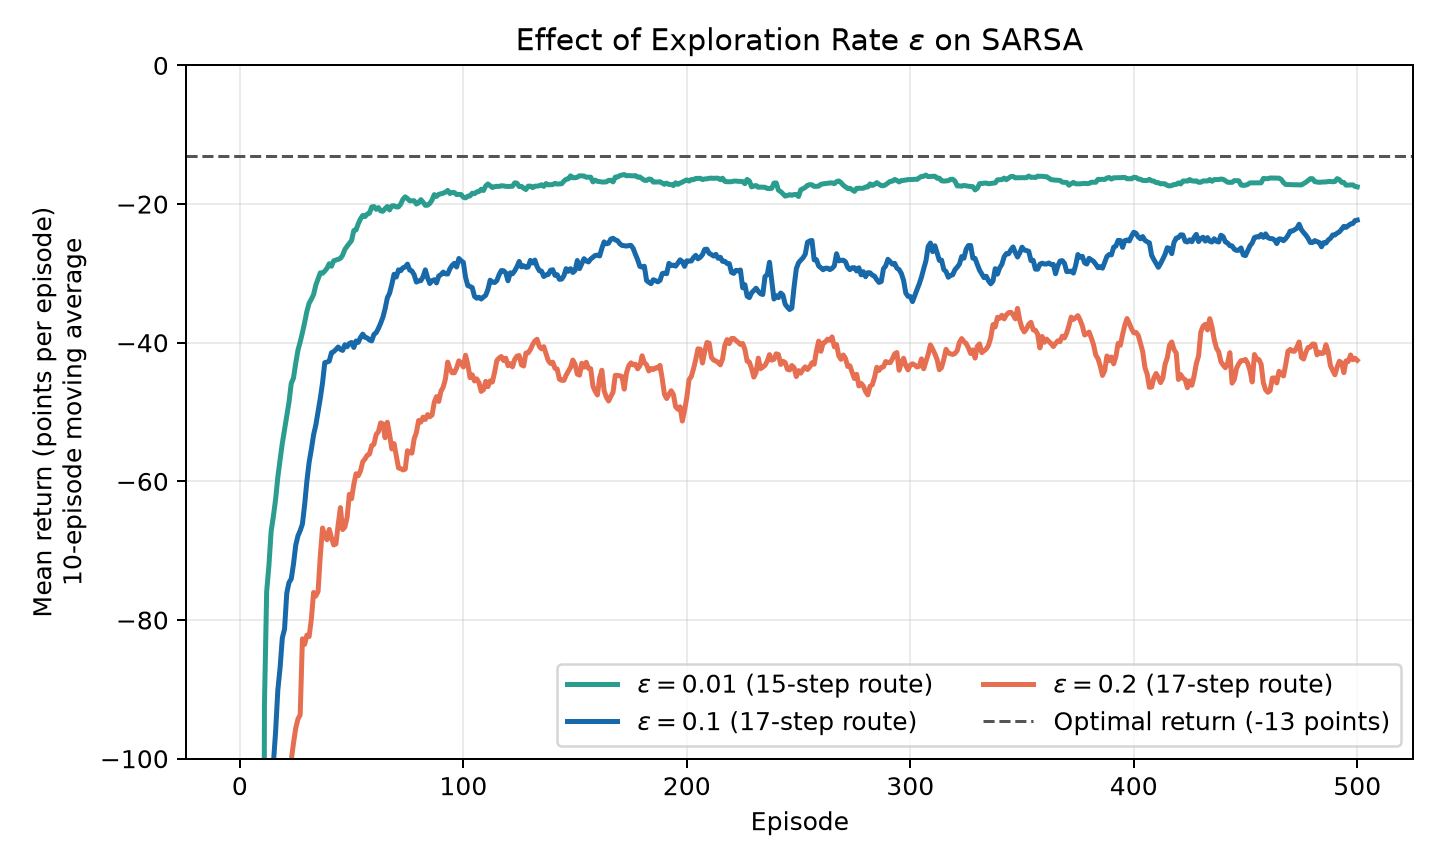
\includegraphics[width=0.92\linewidth]{epsilon_sweep.png}
  \caption{Mean learning curves for the three exploration rates.  All curves
  average the same 50 seeds and use the same 10-episode smoothing window.
  Early values below $-100$ are clipped by the common vertical scale.}
  \label{fig:epsilon}
\end{figure}

\begin{table}[H]
  \centering
  \caption{Comparison with Amaya Bryan's independent execution.  ``Success''
  means that the greedy rollout reached G within its rollout limit.}
  \resizebox{\linewidth}{!}{%
  \begin{tabular}{cccccc}
    \toprule
    $\epsilon$ & Our seed-0 & Mate's seed-0 & Successes & Mean length & Last-100 return \\
    \midrule
    0.01 & 15 & 15 & 49/50 & 15.65 & $-16.86$ \\
    0.10 & 17 & 17 & 44/50 & 17.00 & $-25.16$ \\
    0.20 & 17 & 17 & 28/50 & 17.07 & $-42.93$ \\
    \bottomrule
  \end{tabular}
  }
  \label{tab:lengths}
\end{table}

The two implementations produced the same seed-0 path and the same summary
statistics.  For the default run, both obtained a mean return of $-1725.3$ in
episode 1, $-311.1$ over the first ten episodes, and $-25.16$ over the final
100 episodes.  Fifteen smoothed points were below the plot's $-100$ lower
limit.  The agreement is expected because both programs use the same
environment rules, exact tie detection, NumPy random generator, and seeds.
The comparison also strengthens the qualitative result: as $\epsilon$
increases, fewer final greedy policies reach G after only 500 training
episodes and the online return becomes more negative.  Across the 50 seeds,
crossings also shift away from row 2 toward rows 1 and 0, confirming that
SARSA prices the risk created by its own exploratory behavior.

\section{Discussion Questions}

\subsection{Why does the agent avoid the row next to the cliff?}

The path immediately above the cliff is the shortest deterministic route: go
up once, move right across row 2, and go down into the goal, for a return of
$-13$.  SARSA, however, learns the value of the policy it actually follows,
and that policy remains $\epsilon$-greedy during training.  From row 2, a
random exploratory down action can enter the cliff, produce $-100$, and send
the agent back to the start.  That costly possibility is included in the
bootstrapped value of nearby state--action pairs.  Moving through row 1 or row
0 requires extra $-1$ steps, but it provides a buffer: one mistaken downward
move does not immediately cause a fall.  The expected return of this safer
route can therefore exceed that of the geometrically shortest route under
continued exploration.  This is the characteristic on-policy behavior of
SARSA.  The seed-0 greedy policy illustrates the tradeoff by taking 17 steps
and spending most of its crossing far above the cliff.

\subsection{How does the route change with $\epsilon$? What happens as
$\epsilon\to0$?}

In this experiment, seed 0 learned a 15-step greedy route at
$\epsilon=0.01$, compared with 17 steps at both $\epsilon=0.1$ and
$\epsilon=0.2$.  The result follows the expected tendency: as exploration
becomes more frequent, positions near the cliff become more expensive because
there are more opportunities for an accidental downward move.  SARSA folds
that risk into its on-policy action values, so larger $\epsilon$ favors a wider
safety margin, even when the resulting greedy path contains additional
steps.  The learning curves also show the direct performance cost of random
actions: $\epsilon=0.2$ has substantially lower returns than $\epsilon=0.1$,
whereas $\epsilon=0.01$ remains closest to the optimal-return reference.  As
$\epsilon$ approaches zero, a sufficiently trained and sufficiently explored
agent should favor the 13-step route along row 2 because cliff risk vanishes
during execution.  Exactly $\epsilon=0$ is different: without prior
exploration, early random tie choices can leave useful actions insufficiently
sampled, so convergence to the optimal route is not guaranteed.

\subsection{Which line makes the algorithm on-policy?}

The decisive operations are lines 95 and 97 of
\texttt{cliff\_walk\_sarsa.py}.  Line 95 samples
\texttt{next\_action} from the same $\epsilon$-greedy behavior policy that is
used to interact with the environment.  Line 97 then places the value of that
specific sampled action in the target:
\[
\texttt{target = reward + GAMMA *
q\_values[next\_row, next\_col, next\_action]}.
\]
Finally, the assignment
\texttt{state, action = next\_state, next\_action} executes that same sampled
action on the following iteration.  Thus the update evaluates the action the
agent will actually take, including exploratory choices.  This is precisely
the on-policy property of SARSA.  If the target instead used
$\max_a Q(S_{t+1},a)$, it would evaluate a greedy target policy while behavior
remained $\epsilon$-greedy; that would be the off-policy Q-learning update.
For terminal transitions the target is just the observed reward because no
next action exists, which does not alter the on-policy distinction.

\section{Reproducibility}

Run the experiment from this directory with:
\begin{verbatim}
python cliff_walk_sarsa.py
\end{verbatim}
The script recreates all three files under \texttt{figures/} and prints the
three route lengths and the default seed-0 route.

\end{document}
